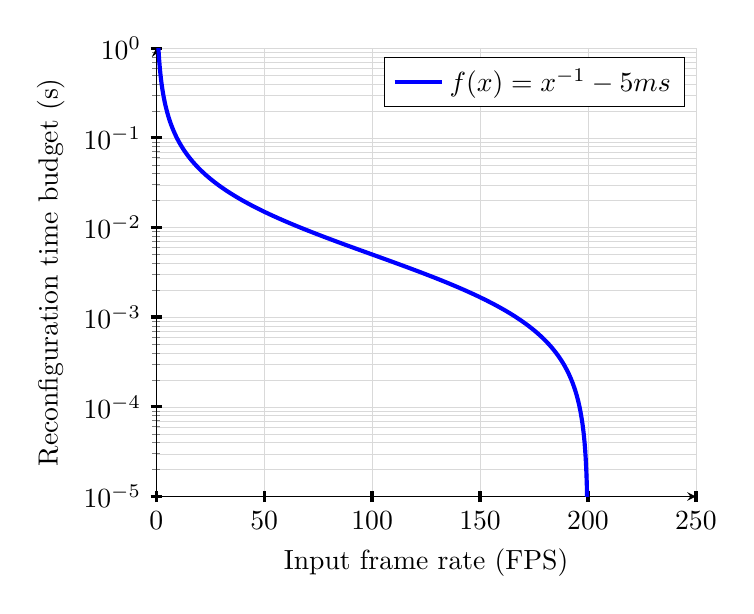
\begin{tikzpicture}
\begin{semilogyaxis}[
    xmin=0, xmax=250,
    ymin=0.00001, ymax=1,
    axis lines = left,
    xlabel = {Input frame rate (FPS)},
    ylabel = {Reconfiguration time budget (s)},
    ymajorgrids=true,
    grid=both,
    % grid style=dashed,
    grid style={line width=.1pt, draw=gray!30},
    every major tick/.append style={very thick, major tick length=4pt, black},
]

% 16 bits
\addplot[
    domain=0:250, 
    samples=1000, 
    color=blue,
    line width=1.5pt
]
{1/x - 0.005};
% \addlegendentry{$B(f) = f^{-1} - \SI{5}{ms}$}
\addlegendentry{$f(x) = x^{-1}  - \SI{5}{ms}$}
\end{semilogyaxis}
\end{tikzpicture}
